\section* {1.2  Метод прогонки}

\subsection{Постановка задачи}
Реализовать метод прогонки в виде программы, задавая в качестве входных данных ненулевые элементы матрицы системы и вектор правых частей. Используя разработанное программное обеспечение, решить СЛАУ с трехдиагональной матрицей.  

{\bfseries Вариант:} 22

\begin{cases}
& -14x_1+6x_2 = 82 \\
& 2x_1+7x_2 = -51 \\
& -7x_2-18x_3-9x_4 = -46 \\
& 2x_3-13x_4+2x_5 = 111 \\
& -7x_4-7x_5 = 35 \\
\end{cases}
% \pagebreak

\subsection{Результаты работы}
\begin{figure}[h!]
\centering
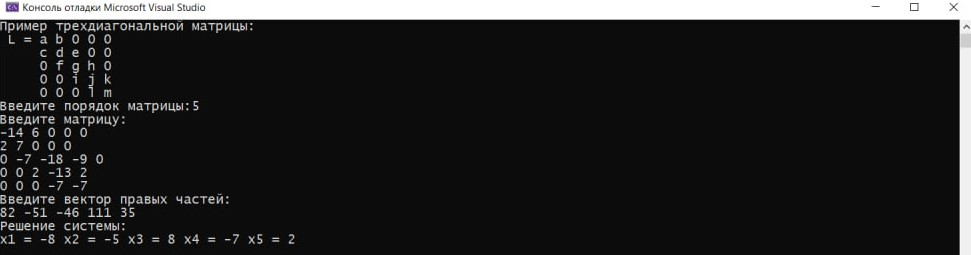
\includegraphics[width=.9\textwidth]{lab1.2}
\caption{Вывод программы в консоли}
\end{figure}

% \vfill

% \begin{figure}[h!]
% \centering
% 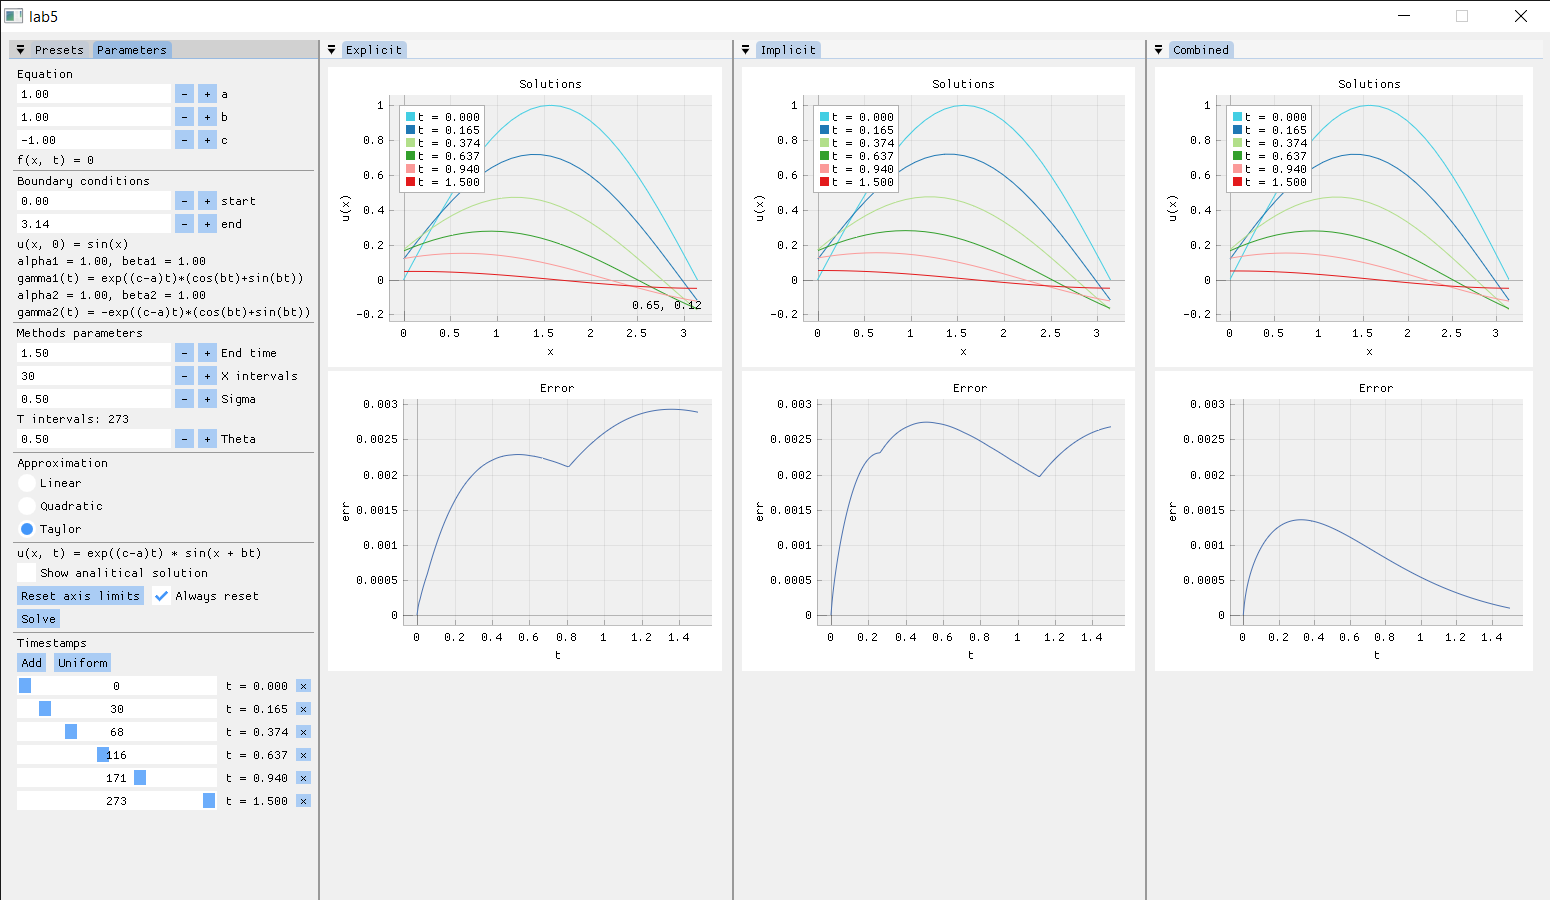
\includegraphics[width=.9\textwidth]{lab5_taylor}
% \caption{Решение с аппроксимацией граничных условий со вторым порядком}
% \end{figure}
\pagebreak

\subsection{Исходный код}
% \lstinputlisting[language=C++]{matrix.cpp}
% \begin{lstlisting}
\lstinputlisting{include/lab1_2.cpp}
\lstinputlisting{include/matrix.cpp}
\lstinputlisting{include/matrix.h}
% \end{lstlisting}
% \lstinputlisting{matrix.cpp}
% {../../include/matrix.cpp}
% \pagebreak
% \lstinputlisting[title=\texttt{parabolic\_pde.hpp}]{../../include/partial_differential/parabolic_pde.hpp}
% \pagebreak
% 